\nofiles
\documentclass[crop,tikz]{standalone}
\usepackage{amsmath}
\usepackage{amssymb}
\usepackage{tikz}
\usepackage{tikz-cd}

\usetikzlibrary{arrows.meta,decorations.pathmorphing}

\begin{document}
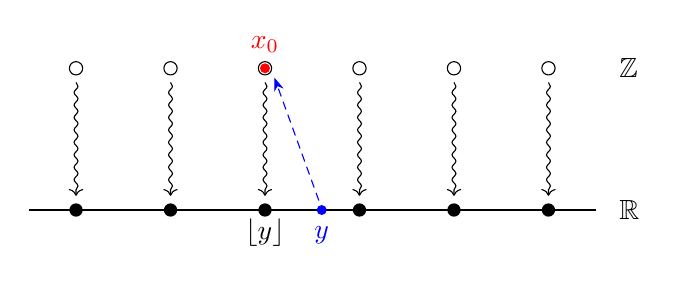
\begin{tikzpicture}[>=Stealth,scale=1.2]

  % Real line
  \draw[thick] (-0.5,0) -- (5.5,0);
  \node[right,xshift=5pt] at (5.5,0) {$\mathbb{R}$};

  % Z row of hollow dots and squiggly arrows
  \foreach \i in {0,...,5} {
    \draw (\i,1.5) circle (2pt); % hollow Z dot
    \fill (\i,0) circle (2pt);               % filled R dot
    \draw[->,>=To,decorate,decoration={snake,amplitude=0.7,segment length=4.5}]
         (\i,1.35) -- (\i,0.15); % squiggle arrow
  }
  % Label Z
  \node[right,xshift=5pt] at (5.5,1.5) {$\mathbb{Z}$};

  % A blue point on the real line (say 2.6)
  \fill[blue] (2.6,0) circle (1.5pt) node[below,yshift=-2.5pt]{$y$};

  \node[below,yshift=0.5pt] at (2, 0) {$\lfloor y \rfloor$};

  % Circle the Z=2 dot
  \fill[red] (2,1.5) circle (1.5pt) node[above,xshift=0pt,yshift=2pt]{$x_0$};

  % Arrow from y to 2
  \draw[->,blue, dash pattern=on 3pt off 2pt] (2.57,0.1) to (2.1,1.4);

\end{tikzpicture}
\end{document}